\documentclass[a4paper]{article}

\usepackage{color}
\usepackage{url}
\usepackage[T2A]{fontenc} 
\usepackage[utf8]{inputenc}
\usepackage{graphicx}

\usepackage[english,serbian]{babel}
\usepackage[unicode]{hyperref}
\hypersetup{colorlinks,citecolor=red,filecolor=green,linkcolor=blue,urlcolor=blue}

\title{Slučajevi upotrebe Udruženja u okviru zaposlenih}


\begin{document}

\maketitle

\section{Slučajevi upotrebe}

\subsection{Udruženja}
\subsubsection{Slučaj upotrebe: Zahtev za prisustvo događaju}
\begin{enumerate}
    \item \textbf{Kratak opis:} Zaposleni u kompaniji šalje zahtev za prisustvo događaju organizovanom od strane već postojeće zajednice u kompaniji.
    \item \textbf{Učesnici:}
        \begin{itemize}
            \item Zaposleni
        \end{itemize}
    \item \textbf{Preduslovi:} Sistem je u funkciji. Zaposleni ima pristup internetu, sistemu.
    \item \textbf{Postuslovi:} Zaposleni se uspešno prijavio za prisustvo događaju. Vlasnik zajednice je obavešten.
    \item \textbf{Osnovni tok:}
        \begin{enumerate}
            \item Zaposleni otvara stranicu za udruženja.
            \item Sistem prikazuje listu svih postojećih udruženja
            \item Zaposleni otvara stranicu udruženja za čiji događaj je zainteresovan
            \item Zaposleni otvara stranicu svih događaja udruženja
            \item Zaposleni bira događaj kome želi da prisustvuje
            \item Zaposleni se prijavljuje za događaj pritiskom na dugme Želim da Prisustvujem
            \item Sistem prikazuje da je prijava uspešna 
        \end{enumerate}
    \item \textbf{Alternativni tokovi:}
        \begin{enumerate}
            \item \textbf{Prijave za događaj su zatvorene.} Sistem obaveštava korisnika da je prijavljivanje zatvoreno. Sistem vraća korisnika na korak (d)
        \end{enumerate}
    \item \textbf{Podtokovi:} /
    \item \textbf{Specijalni zahtevi:} /
    \item \textbf{Dodatne informacije:} /
\end{enumerate}

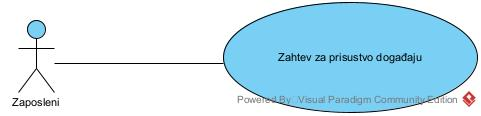
\includegraphics[scale=0.5]{UML/SlucajUpotrebe_PrisustvoDogadjaju.jpg}

\end{document}